\subsection{Parametric Curves}

Describe a curve by 2+ functions and a variable $t$.

\begin{example}
$\ve{x(t),\, y(t)} = \ve{2t,\, 3t-1}$, \quad $-2 \le t \le 3$

\begin{center}
\begin{tikzpicture}
\begin{axis}[
    axis lines=middle,
    xlabel=$x$, ylabel=$y$,
    xmin=-6, xmax=8, ymin=-9, ymax=9,
    xtick={-4,-2,...,6}, ytick={-8,-4,4,8},
    width=8cm, height=7cm,
    samples=50,
]
\addplot[thick, domain=-2:3, ->] ({2*x},{3*x-1});
\addplot[only marks, mark=*] coordinates {(-4,-7) (6,8)};
\end{axis}
\end{tikzpicture}
\end{center}

Eliminating the parameter: from $x = 2t$ we get $t = x/2$, so
\[
    y(t) \leftarrow ...x(t) \qquad\Longrightarrow\qquad
    y = \tfrac{3}{2}\,x - 1.
\]
\end{example}

\begin{example}
$\ve{x(t),\, y(t)} = \ve{t^{2},\, t^{3}}$, \quad $-2 \le t \le 2$

\begin{center}
\begin{tikzpicture}
\begin{axis}[
    axis lines=middle,
    xlabel=$x$, ylabel=$y$,
    xmin=-1, xmax=5, ymin=-9, ymax=9,
    xtick={1,2,3,4}, ytick={-8,-4,4,8},
    width=8cm, height=8cm,
    samples=100,
]
\addplot[thick, variable=t, domain=-2:2] ({t^2},{t^3});
\addplot[only marks, mark=*] coordinates {(4,-8) (4,8)};
\end{axis}
\end{tikzpicture}
\end{center}
\end{example}

\begin{example}[Cycloid]
A circle of radius 1 rolls along the $x$-axis. Track a point $P$ on its rim.

\begin{center}
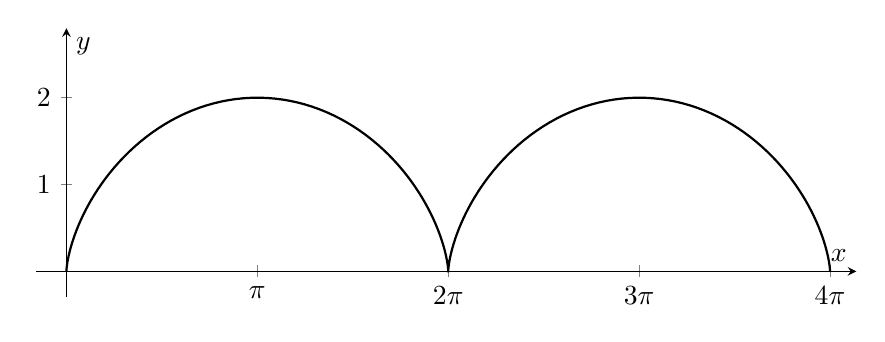
\begin{tikzpicture}
\begin{axis}[
    axis lines=middle,
    xlabel=$x$, ylabel=$y$,
    xmin=-0.5, xmax=13, ymin=-0.3, ymax=2.8,
    width=12cm, height=5cm,
    samples=200,
    xtick={3.14159,6.28318,9.42478,12.5664},
    xticklabels={$\pi$,$2\pi$,$3\pi$,$4\pi$},
    ytick={1,2},
]
\addplot[thick, variable=t, domain=0:4*pi]
    ({t - sin(deg(t))},{1 - cos(deg(t))});
\end{axis}
\end{tikzpicture}
\end{center}

Let center $C = (t,\,1)$. Then
\[
    P\ve{x(t),\,y(t)}
    = \ve{t,\,1} + \ve{-\sin t,\;-\cos t}
    = \ve{t - \sin t,\; 1 - \cos t}.
\]
\end{example}

\subsection{Calculus with Parametric Curves}

\subsubsection*{Chain Rule}

\[
    \frac{dy}{dx}
    = \frac{dy/dt}{dx/dt}
    = \frac{y'}{x'}
\]

\begin{example}
$\ve{x,y} = \ve{2t,\, 3t-1}$:
\[
    \frac{dy}{dx} = \frac{y'}{x'} = \frac{3}{2}
\]
\end{example}

\begin{example}
$\ve{x,y} = \ve{t^{2},\, t^{3}}$:
\[
    \frac{dy}{dx} = \frac{y'}{x'} = \frac{3t^{2}}{2t} = \frac{3}{2}\,t
\]

Tangent line at $P = (4,\,-8)$ \; ($t = -2$):
\[
    \left.\frac{dy}{dx}\right|_{t=-2} = -3
    \qquad\Longrightarrow\qquad
    y - (-8) = -3(x - 4)
\]

\begin{center}
\begin{tikzpicture}
\begin{axis}[
    axis lines=middle,
    xlabel=$x$, ylabel=$y$,
    xmin=-1, xmax=5, ymin=-12, ymax=9,
    width=7cm, height=8cm,
    samples=100,
]
\addplot[thick, variable=t, domain=-2:2] ({t^2},{t^3});
\addplot[dashed, domain=1:5] {-3*(x-4)-8};
\addplot[only marks, mark=*] coordinates {(4,-8)};
\end{axis}
\end{tikzpicture}
\end{center}
\end{example}

\subsubsection*{Second Derivatives}

\[
    \frac{d^{2}y}{dx^{2}}
    = \frac{d}{dx}\!\left(\frac{dy}{dx}\right)
    = \frac{1}{x'}\,\frac{d}{dt}\!\left(\frac{y'}{x'}\right)
    = \frac{y''x' - x''y'}{(x')^{3}}
\]

\begin{example}
$\ve{x,y} = \ve{t^{2},\, t^{3}}$: \quad $x' = 2t$, $x'' = 2$, $y' = 3t^{2}$, $y'' = 6t$.
\[
    \frac{d^{2}y}{dx^{2}}
    = \frac{6t\cdot 2t - 2\cdot 3t^{2}}{(2t)^{3}}
    = \frac{6t^{2}}{8t^{3}}
    = \frac{3}{4t}
\]
\end{example}

\subsubsection*{Arc Length}

\[
    L = \int_{t_{1}}^{t_{2}} \sqrt{x'^{2} + y'^{2}} \dd{t}
\]

\begin{example}[Circle]
$P\ve{x,y} = \ve{\cos t,\, \sin t}$:
\[
    \text{Circumference}
    = \int_{0}^{2\pi}\sqrt{(-\sin t)^{2}+(\cos t)^{2}}\dd{t}
    = \int_{0}^{2\pi} 1\dd{t}
    = 2\pi
\]
\end{example}

\begin{example}[Astroid]
$\ve{x,y} = \ve{\cos^{3}t,\, \sin^{3}t}$ --- circle but shrunk.

\begin{center}
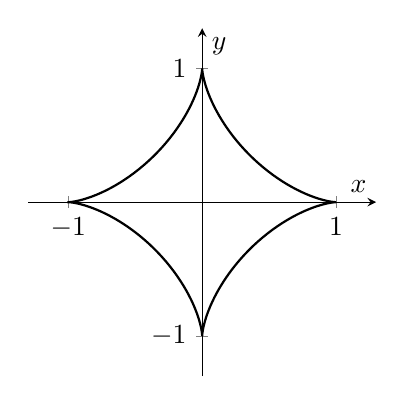
\begin{tikzpicture}
\begin{axis}[
    axis lines=middle,
    xlabel=$x$, ylabel=$y$,
    xmin=-1.3, xmax=1.3, ymin=-1.3, ymax=1.3,
    width=6cm, height=6cm,
    samples=200,
    axis equal,
]
\addplot[thick, variable=t, domain=0:360]
    ({cos(t)^3},{sin(t)^3});
\end{axis}
\end{tikzpicture}
\end{center}

By symmetry, circumference $= 4\displaystyle\int_{0}^{\pi/2}
\sqrt{(3\cos^{2}t\,(-\sin t))^{2}+(3\sin^{2}t\,\cos t)^{2}}\dd{t}$.
\begin{align*}
    &= 4\cdot 3\int_{0}^{\pi/2}\cos t\,\sin t\dd{t}
    = 12\int_{0}^{\pi/2}\tfrac{1}{2}\sin 2t\dd{t} \\
    &= -3\cos 2t\,\Big|_{0}^{\pi/2}
    = -3(-1-1) = 6
\end{align*}
\end{example}

\subsection{Polar Coordinates}

Point $P$ has polar coordinates $(r,\theta)$ and Cartesian $(x,y)$.
\[
    (x,y) = (r\cos\theta,\; r\sin\theta)
    \qquad
    r = \sqrt{x^{2}+y^{2}}, \quad
    \theta = \arctan\frac{y}{x} \;\text{(with quadrant fixed)}
\]

\begin{example}
Point $(-3,\,\sqrt{3})$ to polar: \quad
$\theta = \pi + \arctan\dfrac{\sqrt{3}}{-3} = \pi - \dfrac{\pi}{6} = \dfrac{5\pi}{6}$.
\end{example}

\begin{example}
Curve $r = 4\sin\theta$. Multiply both sides by $r$:
\[
    r^{2} = 4r\sin\theta
    \;\Longrightarrow\;
    x^{2}+y^{2} = 4y
    \;\Longrightarrow\;
    x^{2}+(y-2)^{2} = 4
\]

\begin{center}
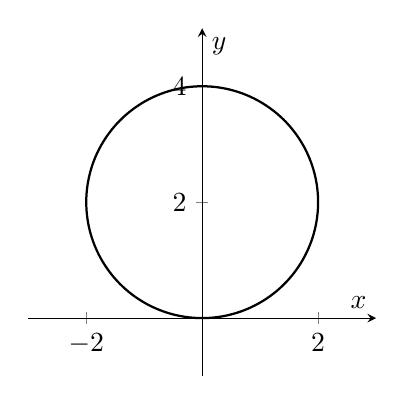
\begin{tikzpicture}
\begin{axis}[
    axis lines=middle,
    xlabel=$x$, ylabel=$y$,
    xmin=-3, xmax=3, ymin=-0.5, ymax=4.5,
    width=6cm, height=6cm,
    samples=200,
    axis equal,
]
\addplot[thick, variable=t, domain=0:360]
    ({4*sin(t)*cos(t)},{4*sin(t)*sin(t)});
\end{axis}
\end{tikzpicture}
\end{center}
Circle centered at $(0,2)$ with radius $2$.
\end{example}

\subsubsection*{Derivatives}

Since $x = r(\theta)\cos\theta$ and $y = r(\theta)\sin\theta$:
\[
    \frac{dy}{dx}
    = \frac{dy/d\theta}{dx/d\theta}
    = \frac{r'\sin\theta + r\cos\theta}{r'\cos\theta - r\sin\theta}
\]

\begin{example}[Cardioid]
$r = 2(1-\sin\theta)$, so $r' = -2\cos\theta$.

\begin{center}
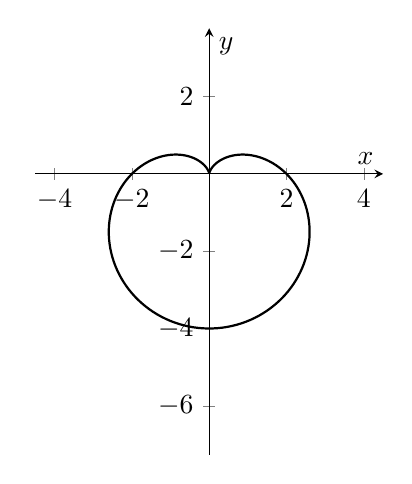
\begin{tikzpicture}
\begin{axis}[
    axis lines=middle,
    xlabel=$x$, ylabel=$y$,
    xmin=-4.5, xmax=4.5, ymin=-5, ymax=1.5,
    width=6cm, height=7cm,
    samples=200,
    axis equal,
]
\addplot[thick, variable=t, domain=0:360]
    ({2*(1-sin(t))*cos(t)},{2*(1-sin(t))*sin(t)});
\end{axis}
\end{tikzpicture}
\end{center}

\begin{align*}
    \frac{dy}{dx}
    &= \frac{-2\cos\theta\sin\theta + 2(1-\sin\theta)\cos\theta}
           {-2\cos^{2}\theta - 2(1-\sin\theta)\sin\theta} \\[4pt]
    &= \frac{\cos\theta\,(1-2\sin\theta)}{2\sin^{2}\theta - \sin\theta - 1}
     = \frac{\cos\theta\,(1-2\sin\theta)}{(\sin\theta - 1)(2\sin\theta + 1)}
\end{align*}

Horizontal tangent (numerator $= 0$, denominator $\neq 0$):
\begin{itemize}[nosep]
    \item $\cos\theta = 0$: $\theta = \frac{\pi}{2}$ \xmark, \;
          $\theta = \frac{3\pi}{2}$ \checkmark
    \item $1 - 2\sin\theta = 0$: $\theta = \frac{\pi}{6}$ \checkmark, \;
          $\theta = \frac{5\pi}{6}$ \checkmark
\end{itemize}

Vertical tangent (denominator $= 0$, numerator $\neq 0$):
\begin{itemize}[nosep]
    \item $\sin\theta - 1 = 0$: $\theta = \frac{\pi}{2}$ \xmark
    \item $2\sin\theta + 1 = 0$: $\theta = \frac{7\pi}{6}$ \checkmark, \;
          $\theta = \frac{11\pi}{6}$ \checkmark
\end{itemize}

At $\theta = \frac{\pi}{2}$ both vanish --- take the limit:
\[
    \lim_{\theta\to\pi/2^{+}} \frac{dy}{dx}
    = \lim_{\theta\to\pi/2}
      \frac{1-2\sin\theta}{2\sin\theta+1}\cdot\frac{\cos\theta}{\sin\theta-1}
    = \frac{-1}{3}\lim_{\theta\to\pi/2}\frac{\cos\theta}{\sin\theta-1}
    \stackrel{\text{L'H}}{=} \frac{-1}{3}\cdot\frac{-\sin\theta}{\cos\theta}
    = \pm\infty
\]
\end{example}

\subsection{Vector Recap}

\begin{itemize}
    \item Zero vector: $\mathbf{0} = \ve{0,\,0}$ in 2D.
    \item Unit vector: magnitude of $1$. \;
          $\dfrac{\mathbf{a}}{\lVert\mathbf{a}\rVert}$ = unit vector in direction of $\mathbf{a}$.
    \item Dot product:
          $\mathbf{a}\cdot\mathbf{b}
          = \ve{a_{1},\,a_{2}}\cdot\ve{b_{1},\,b_{2}}
          = a_{1}b_{1}+a_{2}b_{2}$
    \item $\mathbf{a}\cdot\mathbf{a} = \lVert\mathbf{a}\rVert^{2}$
    \item $\mathbf{a}\perp\mathbf{b} \;\Longleftrightarrow\; \mathbf{a}\cdot\mathbf{b} = 0$
\end{itemize}

\subsubsection*{Projection of $\mathbf{a}$ onto $\mathbf{b}$}

\begin{center}
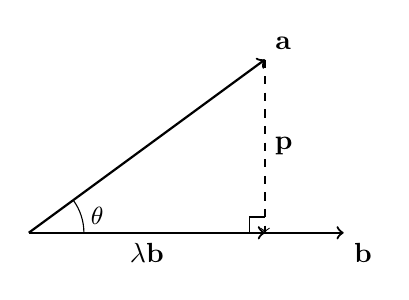
\begin{tikzpicture}
\coordinate (O) at (0,0);
\coordinate (B) at (4,0);
\coordinate (A) at (3,2.2);
\coordinate (P) at (3,0);
% vectors
\draw[->, thick] (O) -- (B) node[below right]{$\mathbf{b}$};
\draw[->, thick] (O) -- (A) node[above right]{$\mathbf{a}$};
\draw[->, dashed] (A) -- (P) node[midway, right]{$\mathbf{p}$};
\draw[->, thick] (O) -- (P) node[below, midway]{$\lambda\mathbf{b}$};
% angle
\draw (0.7,0) arc[start angle=0, end angle=36, radius=0.7]
    node[midway, right]{\small$\theta$};
% right angle mark
\draw (P) ++(0,0.2) -- ++(-0.2,0) -- ++(0,-0.2);
\end{tikzpicture}
\end{center}

Let $\lambda\mathbf{b} \parallel \mathbf{b}$ and $\mathbf{p}\perp\mathbf{b}$, so that $\mathbf{a} = \lambda\mathbf{b} + \mathbf{p}$.
\begin{align*}
    \lVert\mathbf{a}\rVert^{2}
    &= \lVert\lambda\mathbf{b}\rVert^{2} + \lVert\mathbf{p}\rVert^{2} \\
    \lVert\mathbf{a}\rVert^{2}
    &= \lambda^{2}\lVert\mathbf{b}\rVert^{2}
     + \lVert\mathbf{a}-\lambda\mathbf{b}\rVert^{2} \\
    a^{2} &= \lambda^{2}b^{2} + (\mathbf{a}-\lambda\mathbf{b})^{2}
\end{align*}
\[
    \Longrightarrow\quad
    \lambda = \frac{\mathbf{a}\cdot\mathbf{b}}{\lVert\mathbf{b}\rVert^{2}}
    \qquad\Longrightarrow\quad
    \lVert\lambda\mathbf{b}\rVert
    = \lambda\lVert\mathbf{b}\rVert
    = \lVert\mathbf{a}\rVert\cos\theta
\]

$\text{comp}_{\mathbf{u}}\,\mathbf{v}
= \dfrac{\mathbf{u}\cdot\mathbf{v}}{\lVert\mathbf{u}\rVert}$
\; --- scalar projection of $\mathbf{v}$ onto $\mathbf{u}$ (signed length).
